\chapter{Background} \label{background}

In this chapter, we will look at the fundamental concepts and theory for the different diffusion models, seed selection algorithms and performing BFS over boolean semiring. We will also have a look at HLS and specifications of the Zedboard. This chapter will contain notations that we will use throughout the report.

 We will look at the independent cascade model, which is a special case of breadth first search  \cite{HybridBFS2015}. By looking at how to improve BFS, we can apply such optimization to ICM and the seed selection algorithm.
 \\

\begin{figure}[!ht]
	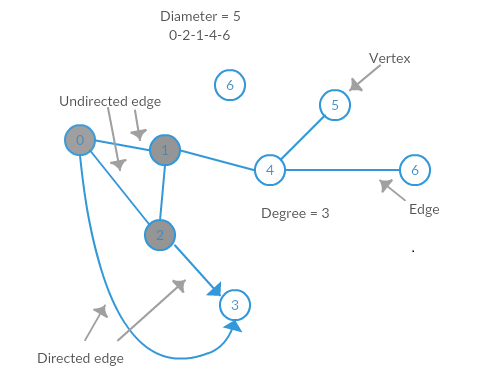
\includegraphics[scale=0.7]{Figures/smallExampleNetwork2}
	\caption{Simple network} 
	\label{fig:SimpleGraph}
\end{figure}

\section{Network Teminalogy and Glossary}
The fundamental unit in a network is a \textit{vertex} (pl. vertices), sometimes called a node. For this report, vertex will be used. The connecting between two vertices is called an \textit{edge}, and is shown in Figure \ref{fig:SimpleGraph}. Different networks have different types of edges, some are\textit{directed}, while others are \textit{undirected}. A directed edge is an edge that runs in only one direction (such as a one-way road between two points), and undirected runs in both directions. Directed edges can be recognised as an arrow to indicating their orientation, while undirected edges have no orientation. 

Each vertex has a value that is called \textit{degree}. Degree for a vertex $v_1$ is the amount of edges connected to $v_1$. Note that the degree is not necessarily equal to the number of vertices adjacent to a vertex, since there may be more than one edge between two vertices. A vertex with directed edges has both an in-degree and an out-degree, which are the numbers of in-coming and out-going edges respectively. The \textit{component} to which a vertex belongs is that set of vertices that can be reached from it by paths running along edges of the graph. In a directed graph a vertex has both an in-component and an out-component, which are the sets of vertices from which the vertex can be reached and which can be reached from it.

A \textit{geodesic path} is the shortest path through the network from one vertex to another. There may be, and often is , more than one geodesic path between two vertices. The \textit{diameter} of a network is the length (in number of edges) of the longest geodesic path between any two vertices. 

\section{Network}
A \textit{network} is a collection of vertices and edges \cite{ComplexNetwork2003}. Many system takes the form of networks, e.g. the internet, the World Wide Web, social media sites suxh as Facebook, Twitter, Gihub, etc. These networks  can be categorized into different types, e.g. \textit{social networks} \cite{ComplexNetwork2003}, \textit{information networks} \cite{ComplexNetwork2003}, \textit{technological networks} \cite{ComplexNetwork2003} ,and \textit{biological networks} \cite{ComplexNetwork2003}. Different networks have different properties and in this report we will look at those most relevant to social networks.

\subsection{Social Network}
A social network is a set of individuals connected to each other via some form of contact or interactions \cite{ComplexNetwork2003}. The vertices are people and the edges are teh connections between people. The social network display information regarding connection, interaction or location of a set of people. It forms patterns regarding friendships, business interactions between companies and families history. The social network is often used in social science \cite{ComplexNetwork2003}. Some notable experiments are the letter passing experiment \cite{smallWorldExperiment1969}, which we will discuss more in Section \ref{sec:SmallWorldeffect} 

\section{Network Properties}
\textit{Network properties} are different characteristic traits that networks display. We will focus on those that are the most relevant to social networks and their relevance to ICM, data diffusion and seed selection.


\subsection{The Small World Effect} \label{sec:SmallWorldeffect}
The small world effect was first demonstrated by Stanley Milgram in the 1960s during his famous letter passing experiment \cite{SmallWorldProblemSmilgram1960}. The experiment involved passing letters from person to person to reach a designated target with only small steps. For the published case, the chain was around six\cite{Experiment1969}, meaning there were only six passes necessary for the letter to reach its destination. This shows us that most pairs of vertices in a network can reach each other with a short path. A more precise wording is that "Networks are said to show the small world effect if the value of \textit{l} scales logarithmic or slower with the network size for a fixed mean degree." \cite{ComplexNetwork2003}. We have defined \textit{l}  to be the mean geodesic distance between vertex pairs in a network.

For the data diffusion problem, this kind of effect would result in that the diffusion through a network would need around 6 steps to have travelled through the entire network if the transition probability is high. Meaning that most node can reach each other through a relatively small step.

\subsection{Transitivity/Clustering}
In networks, there is often a special connection pattern called \textit{triangles}. Triangles is where three Vertices : $v_a,v_b,v_c$ is all connected to each other as shown in Figure \ref{fig:triangleStruc}. We can look at such a connection as person A is friends with B and C, and B and C are friends with each other too. Transitivity is used to determine how many triangles is present in the network.  

\begin{figure}
	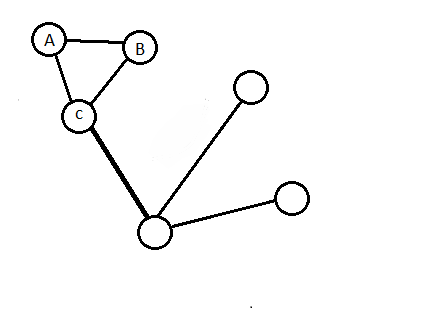
\includegraphics{Figures/triangleStruc}
	\caption{Examples of triangles in networks} 
	\label{fig:triangleStruc}
\end{figure}


For data diffusion and seed selection, this would mean that picking nodes that are neighbours to each other, would have a smaller spread then picking two not neighbouring vertices. By picking two nodes that are connected to each other, they would likely share common neighbours and thus having a smaller reach.  

\subsection{Degree Distribution} \label{degreeDis}
As mentioned earlier, each node has a degree. The degree distribution shows how the different degrees in the network is distributed and how many nodes have a specific degree. Different networks have different shaped degree distribution.

For random graphs, the distribution would most likely be a \textit{Poiison distribution} or \textit{binomial}\cite{ComplexNetwork2003}. For social graph, the degree distribution is often in the shape of exponential distribution. For the information diffusion, this distribution shows us how many high degree nodes there are in the network and those node would likely be high prioritized node. One of the algorithm uses the distribution to select the seed nodes. We will discuss this in later sections.  

%Skrive om hva forskjellige distributuon handler om. 


\subsection{Degree Correlations} \label{degreeCorr}
As mentioned in Section \ref{degreeDis}, networks has a degree distribution with few high degree nodes and many low degree nodes. One interesting property is the degree correlation. Degree correlations is how the high degree and low degree nodes connects to each other. One question is wether high degree nodes tends to connect to other high degree nodes, or if they prefer to connect to low degree nodes. It turns out that both incidents are found in networks \cite{ComplexNetwork2003}. Most social networks are assortative, meaning vertices have a selective linking, where high degree verticies tends to connect to other high degree verticies. Technological network and biological network are most likely disassortative \cite{AssortativeMixing2002}. 

For information diffusion, this kind of behaviour would result in wasting a seed by picking a majority of high degree nodes for starting seed, since most of them would be connected to each other. One solution is by mixing the selection, choose some percentage to be high degree, and some with lower degree.

\subsection{Network Resilience}
For most network model, there is the need to remove nodes from the network. Removal of a node can have no effect on the network, or it can be devastating. \textit{Network resilience} looks at how the network resists to such a removal. There are two different removal schemes, the random removal where nodes are randomly picked and removed, or the targeted removal where specific nodes are removed depending on the criteria. 

The experiment mentioned in \cite{ComplexNetwork2003} by Albert et al showed that for a subset of networks representing the Internet and the World Wide Web, targeted removal had a larger impact than random removal. The random removal had a minimal effect on the network, while the targeted removal had a much larger impact, where mean vertex-to-vertex distance increased. They proposed that the internet was highly resilient to random removal, while much more vulnerable to targeted removal. 

In the case of information diffusion, a targeted removal would result in massive change to the diffusion path. By removing a high degree node it would result in the removal of influential nodes and limit the spread of data. Removing important nodes connecting two different communities would result in isolation and no path towards other communities. In our case, we assume that the network is a static, unchanging network. 

\subsection{Community Structure}
One property that is often observed in a social network, is the community structure. The community structure is where a group of vertices having a high density of edges between each other, while having low density of edges to other communities. We can see an example of the community structure clearly displayed from \cite{RaceInSchool}, where we can see the playground was divided into different communities.

This type of community structure would have a large impact on how the algorithm would select a seed for information diffusion. If all the seeds would be selected in one community, the probability of spreading over to other communities would be smaller. This is of course dependent on how many intercommunity connections there are in within the network.



\begin{list}{1}
\item what is Information diffusion
\item what is the solution(bfs)
\item what is ICM
\item how to implement bfs as SpMV
\item how to apply information diffusion to bfs and problem
\item 
\end{list}

